\section{فصل دوم، درک دامنه و جمع‌آوری نیازمندی‌ها}

این فصل معادل فاز (فرایند) اول مهندسی نیازمندی یعنی استخراج داده‌ها می‌باشد.
تمام مشکلاتی که در \lr{Scope} می‌باشد در حقیقت \lr{System as is} را مشخص می‌کند.

\subsection{دسته‌بندی جمع‌آوری داده}

جمع‌آوری داده‌ها را می‌توانیم به دو دسته زیر تقسیم کنیم، (درک دامنه و جمع‌آوری
داده‌ها ترکیبی از تکنیک‌های متفاوت می‌باشد):

\begin{enumerate}
    \item تکنیک‌های فرآورده‌گرا یا \lr{Artifact driven}: هر آن چیزی که در پروژه
    تولید یا استفاده می‌شود.
    \item \begin{enumerate}
        \item می‌توانیم از قواعد آموزشی نیازمندی‌هایی را خارج کنیم.
        \item \lr{Prototype}ها
        \item مستندات موجود در سازمان‌ها
    \end{enumerate}
    \item تکنیک‌های ذینفع‌گرا یا \lr{Stakeholder driven}: هر آن چیزی که در
    ارتباط با آدم‌ها در سازمان باشد.
    \item \begin{enumerate}
        \item جلسات
    \end{enumerate}
\end{enumerate}

\subsection{تکنیک‌های جمع‌آوری اطلاعات فرآورده‌گرا}

\subsubsection{\lr{Background study}}

\begin{itemize}
    \item سازمان: نمودار‌های سازمانی، بیزینس پلن‌ها، گزارش‌های مالی، صورتجلسه
    \footnote{\lr{Meeting minutes}}
    \item دامنه‌ها: کتاب‌ها، نظرسنجی‌ها، مقالات، مقررات و استاندارد‌ها،
    گزارش‌های سیستم‌های مشابه در دامنه مشابه
    \item سیستم کنونی یا \lr{System as is}: جریانات کاری مستند شده، فرایند‌ها،
    قوانین بیزینسی، مستندات مبادله شده، گزارش‌های مربوط به شکایات، مستندات مربوط
    به تغییر خواسته‌های مشتری و غیره.
\end{itemize}

یکی از نیازمندی‌های مهم برای ذینفعان می‌باشد تا آن‌ها را نسبت به جلسه بعدی‌شان
آماده کند.

مهم‌ترین مشکلات:

\begin{enumerate}
    \item حجم مستندات به شدت زیاد است
    \item جزئیات نامرتبط برای مثال بخش بایگانی اسنادی را نگهداری می‌کند که ممکن
    است کاملاً با یکدیگر نامرتبط باشد.
    \item اسناد ممکن است منسوخ شده یا \lr{Outdated} باشند.
\end{enumerate}

راه حل مشکلات این بخش:

استفاده از تکنیک هرس کردن مستندات می‌باشد. بررسی بخش‌هایی که معتبر است و حذف
بخش‌هایی که منسوخ شده و غیرمعتبر می‌باشد. این تکنیک مانند خواندن فصل‌های مشخص
شده از یک درس می‌باشد تا اینکه کل فصل‌های مطرح شده را بخواند.

\subsubsection{\lr{Data collection, questionnaires}}

جمع‌آوری داده‌هایی که مستندسازی نشده‌اند. مانند حقایق و ارقام. حقایق و ارقام به
صورت صریح در مستندات موجود نیستند. این داده‌ها می‌تواند به صورت \lr{Meta data}
با شد مانند فرم ثبت‌نام، جمله ندارد بلکه براساس داده‌ها می‌توان به یک جمله رسید.
بر اساس داده‌هایی که جمع‌آوری کرده‌ایم می‌توانیم جملات \lr{Functional} بنویسم.
نوشتن جمله و تفسیر توسط مهندس نیازمندی‌ها بر اساس داده‌های جمع‌آوری شده انجام
می‌پذیرد.

این داده‌ها مانند موارد زیر می‌باشد:

\begin{itemize}
    \item داده‌های مربوط به دیجیتال مارکتینگ، آمار استفاده، ارقام اجرایی و
    عملکردی، هزینه‌ها
    \item استفاده از تکنیک‌های نمونه‌گیری آماری
\end{itemize}

\subsubsection*{مشکلات}

\begin{itemize}
    \item ممکن است تفسیر مهندس نیازمندی لزوماً درست نباشد.
    \item داده کاوی مطمئن و درست ممکن است بسیار زمانبر باشد.
\end{itemize}

در روش قبل که اسنادی که می‌خواندیم اسناد عملیاتی بودند اما در این روش اسنادی که
مطالعه می‌شود کاملاً غیرعملیاتی هستند (مانند معیار‌ها و کیفیت ارائه سرویس).

\subsubsection*{روش‌های احتمالی}

\begin{itemize}
    \item \lr{requirement elicitation}
    \item \lr{Text mining}
\end{itemize}

\subsubsection*{پرسشنامه}

لیستی از سوالاتی که توسط ذینفعان مشخص شده را آماده می‌کنیم که هر کدام یک جواب
مناسب را می‌تواند در برگیرد.

نمونه‌ها میتواند:

\begin{itemize}
    \item انتخاب یک گزینه از چند گزینه. مانند استفاده از \lr{Radio button}
    \item سوالاتی که وزن‌دار هستند:
    \item \begin{itemize}
        \item کیفی: عالی، خوب، بد
        \item کمی: اعلام مقدار به صورت درصدی
    \end{itemize}
\end{itemize}

\subsubsection*{ویژگی‌های یک پرسشنامه خوب}

\begin{enumerate}
    \item تنوع زیاد کاربران و عدم تمرکز موقعیت مکانی و فرهنگ مختلف که در تمام
    کاربران متغیر می‌باشد. پس برای پوشش تنوع و گوناگونی
    \footnote{\lr{Diversity}} کاربران از پرسشنامه استفاده می‌کنیم.
    \item سریع، ارزان و قابل دسترس از راه دور نیازمندی بسیاری از کاربران را
    جمع‌آوری می‌کنیم.
    \item پرسشنامه‌ای خوب است که روایی و کارایی داشته باشد.
\end{enumerate}

\subsubsection*{تفاوت پایایی و روایی در پرسشنامه‌ها}

یک پرسشنامه خوب باید دو ویژگی پایایی و روایی را به همراه داشته باشد. 

\begin{itemize}
    \item پایایی قابلیت اطمینان پرسشنامه به همراه دقت در اندازه‌گیری می‌باشد.
    یعنی اگر همان پرسشنامه در همان شرایط بخواهد به صورت مجدد صورت گیرد، امتیاز
    یا مقدار حاصل از پرسشنامه هیچ تغییری نخواهد کرد.
    \item روایی به معنای آن است که میزان مطابقت نتایج بدست آمده از پرسشنامه با
    دنیای واقعی به چه اندازه‌ای می‌باشد.
\end{itemize}

\subsubsection{\lr{Repertory grids, Card sorts for concept acquisition}}

جمله مجموعه‌ای از اسم‌ها را با فعل به یکدیگر متصل می‌کند تا یک جمله کامل را
تشکیل دهد. برای مثال جمله «دانشجو باید بتواند درس انتخاب کند.» اسم‌ها به ترتیب،
«دانشجو» و «درس» هستند و فعل این جمله که این دو اسم را به یکدیگر متصل می‌کند
«انتخاب کردن» می‌باشد.

اسم‌ها تبدیل به کارت می‌شوند و تمام کارت‌ها معادل به کلاس هستند. تمام کلاس‌ها در
فضای مسئله بررسی می‌شوند و فضای راه‌حل در حقیقت خروجی ارتباط آنها (جمله) است.
یکی از مثال‌های فضای راه‌حل اتصال به دیتابیس می‌باشد.

\subsubsection*{فضای مسئله}

دقیقاً وضعیت موجود را نمایش می‌دهد. تمام چیز‌هایی که می‌بینیم در حقیقت فضای
مسئله می‌باشد.

\subsubsection*{فضای راه‌حل}

فضای راه‌حل نتیجه ارتباط جملات و کلاس‌ها هستند که طراح مشخص می‌کند.

\subsubsection*{مثال}

برای مثال می‌توان به دانشجو و شماره دانشجویی اشاره کرد. نام و نام خانوادگی،
تاریخ تولد، سال ورودی دانشگاه، رشته ورودی، گرایش رشته و غیره تمام مسائلی هستند
که موجودیت دانشجو را تعریف می‌کنند پس فضای مسئله می‌باشند.

طراح سیستم دانشگاهی با توجه به این فضای‌ مسئله ورودی‌ها را بررسی می‌کند و یک
خروجی برای مشخص کردن یکتا بودن دانشجو تولید می‌کند و آن هم شماره دانشجویی
می‌باشد که یکی از مهم‌ترین فرآورده‌های فضای راه‌حل است.

\subsubsection*{نکات}

\begin{itemize}
    \item کاملاً بستگی به نیاز سیستم دارد که مشخص کنیم یک اسم کلاس باشد یا نه.
    زیرا یک اسم می‌تواند کلاس باشد یا می‌تواند به عنوان ویژگی کلاس دیگری یا
    \lr{Attribute} باشد. برای مثال کتابخانه می‌توان اشاره کرد که اگر بخواهیم
    «کتاب‌ها» و «نویسندگان» را کلاس جداگانه در نظر بگیریم می‌توانیم کوئری‌هایی
    در این بابت داشته باشیم که یک کتاب را چه نویسندگانی تالیف کرده‌اند و یا یک
    نویسنده چه کتاب‌هایی دارد. یا می‌توانیم نیاز سیستم را در این ببینیم که یکی
    از \lr{Attribute}های کتاب نویسنده باشد به جای آن که یک کلاس جداگانه داشته
    باشد.
    \item در حالت کلی می‌توان گفت که قانون سفت و سختی برای تشکیل کلاس از روی
    کارت‌ها وجود ندارد و کاملاً نیاز سیستم مشخص می‌کند که کلاس باشند یا
    \lr{Attribute}.
    \item کلاس با محیط مسئله و طراح همراه می‌باشد
    \item اطلاعات یک محصول از ویژگی‌های کلاس است و دسته‌بندی کردن و کتگوری از
    راه‌حل مسئله
    \item صفات یا \lr{Attribute}ها حاوی اعتبارسنجی هستند. برای مثال دارای محدوده
    هستند، نوع دارند و می‌توانند بیان کننده اندازه و پذیرنده مقدار ورودی باشند.
\end{itemize}

\subsubsection*{ویژگی‌ها و معایب}

\begin{itemize}
    \item ساده و ارزان
    \item خیلی از این جمله‌ها می‌تواند دقت پایینی داشته باشند و نامرتبط باشند.
    حتی ممکن است به اسکوپ ما مربوط نباشند.
    \item افرادی می‌توانند این بخش‌ را مدیریت کنند که اسکوپ را خیلی خوب درک کرده
    باشند.
\end{itemize}

\subsubsection{\lr{Scenarios, Storyboards for problem world exploration}}

سناریو به معنای شرح داستانی است که می‌تواند وضعیت و شرایط کنونی و آینده را تعریف
کند. یعنی تعریف \lr{System-as-is} تا \lr{System-to-be}. فقط شروط، جمله‌ها و سطح
پیچیدگی در سیستم افزایش پیدا می‌کند نیازمند تعریف سناریو‌ها هستیم تا بتوانیم
سیستمی که می‌خواهیم طراحی کنیم را بهتر درک کنیم. برای مثال سناریو انتخاب واحد
دانشجو یا اخذ دانشجوی مهمان حاوی شرایط بسیار گسترده‌ای است که بایستی برای هر
کدام از آنها سناریویی در نظر گرفته شود به همین دلیل اهمیت سناریو بسیار بالا
می‌باشد.

\begin{itemize}
    \item چه کاری یا \lr{What}
    \item چه کسی یا \lr{Who}
    \item چرایی یا \lr{Why}
    \item چه می‌شود اگر این اتفاق در نظر گرفته نشود. یعنی دیدن تمام
    \lr{Exception}ها که \lr{What if} را مشخص می‌کند.
\end{itemize}

سناریو‌ها را با استفاده از نمودار‌های \lr{Sequence} نمایش می‌دهیم که در آن تمام
ابعاد بالا وجود دارد به غیر از بُعد \lr{Why}.

\subsubsection*{انواع سناریو‌ها در کنار یکدیگر}

\subsubsection*{سناریو منفی}

سناریو منفی تمام کار‌هایی است که سیستم نباید انجام دهد.

\subsubsection*{سناریو مثبت}

تمام کار‌ها و رفتار‌هایی که انتظار داریم سیستم انجام دهد.

\subsubsection*{سناریو نرمال}

مجموعه سناریو‌های مثبت و منفی در کنار یکدیگر است. برای مثال دانشجو باید بتواند
انتخاب واحد کند (سناریو مثبت). بدون پرداخت شهریه دانشجو نمی‌تواند انتخاب واحد
انجام دهد (سناریو منفی).

\subsubsection*{سناریو غیرنرمال یا \lr{Abnormal}}

سناریو‌ای است که در آن \lr{Exception}ها مشخص می‌شود. برای مثال، دانشجویی که
شهریه پایه را پرداخت کرده باشد می‌تواند انتخاب واحد را انجام دهد. اگر واحدی را
در ترم گذشته مشروط شده باشد که در گروه درسی اجباری باشد در این صورت بایستی این
ترم آن درس را مجدداً اخذ کند در غیر این صورت انتخاب واحد او در این ترم ناقص
خواهد بود.

در حقیقت سناریو غیرنرمال آینده‌نگری روی سیستم \lr{System-to-be} خواهد بود.

\subsubsection*{نکته}

در سناریو نویسی اول سناریو نرمال نوشته می‌شود و سپس برای آن تمام
\lr{Exception}ها را براساس \lr{What if}ها در نظر می‌گیرند تا سناریو منفی را
تشکیل دهند.

\subsubsection*{مزایا و معایب سناریو‌ها}

\begin{itemize}
    \item در سناریو‌ها بُعد \lr{Why} وجود ندارد.
    \item قصه گفتن سخت است و سطح پیچیدگی بالایی را دارد.
    \item ساده بودن از بزرگترین حسن آن است.
\end{itemize}

\subsubsection{\lr{Prototypes, Mock-ups for early feedback}}

همانطور که در صفحات قبلی هم گفته شد، برای متوجه شدن \lr{RFP} بخشی از درخواست‌ها
را به صورت اسکیس یا \lr{User interface} خیلی کلی طراحی می‌کنیم که کمترین حالت
تعامل را دارد تا مشخص شود آیا تا به اینجا کار درخواست‌های مشتری را متوجه شده‌ایم
و بعد از آن مهندسی‌های نیازمندی با درست بود است یا خیر. بعد از جواب گرفتن
\footnote{\lr{Feedback}} از این قسمت می‌توانیم بخش \lr{UI} را کامل و سپس شروع به
پیاده‌سازی کل سیستم کنیم.

\begin{itemize}
    \item تهیه \lr{Prototype}ها مستقیم‌ترین فرآورده‌ای است که برای استخراج
    نیازمندی‌ها استفاده می‌کنیم. بیشتر در آن نیازمندی‌های عملیاتی یا
    \lr{Functional requirement} دیده می‌شود.
    \item نکته مهم آن است که قابلیت‌هایی ارائه می‌دهیم را به صورت
    \lr{Functional} و طراحی که بابت \lr{Prototype} انجام داده‌ایم را
    \lr{Non-Functional} می‌دانیم.
    \item بیشتر تمرکز این روش برای بحث در مورد نیازمندی‌هایی که گنگ بوده
    می‌باشد.
    \item در این روش کار تقریباً سریع می‌باشد تا بتوانیم چالش‌های سیستم را نشان
    بدهیم و تدابیری برای آن بیاندیشیم.
\end{itemize}

% سرچ شود که سخت افزار می‌تواند اسم prototype را بگیرد یا خیر. استاد میگوید
% testbed.

\subsubsection{\lr{Knowledge reuse: Domain-independent, Domain specific}}

در مورد بازیابی دانشی صحبت می‌کند. هدفش افزایش سرعت جمع‌آوری اطلاعات به وسیله
بازیابی دانش از تجربه‌ها نسبت به سیستم‌های مرتبط است. دانشی مشابه در مورد
سازمان‌ها، دامنه‌ها، جهان مسئله مانند نیازمندی‌ها، فرضیه‌ها، ویژگی دامنه‌ها و
غیره.

\subsubsection*{استفاده از فرآیند‌هایی که قبلاً در سیستم‌های مشابه حضور داشتند}

برای مثال بانکداری‌ها معمولاً مجموعه‌ای از تسک‌ها و نقش‌های مشابه‌ای را دارند که
به صورت پوشا یا \lr{Overlap} می‌باشند. یعنی اگر بانک مرکزی هر تعریفی داشته باشد،
دیگر بانک‌های کشور نیز از همان تعاریف در سیستم‌های خود بدون تغییر و سازگاری
استفاده می‌کنند. چرا که همه چیز در سیستم بانکداری مشابه می‌باشد.

در اینجا هدف بر نمایش دانش می‌باشد که المان‌های دانشی که در آینده تشکیل می‌شوند
را شناسایی کنیم. المان‌های دانشی از جنس زیر هستند:

\begin{itemize}
    \item مفاهیم یا \lr{Concepts}
    \item اهداف یا \lr{Goals}
    \item وظایف یا \lr{Tasks}
    \item افراد یا \lr{Agents}
    \item نیازمندی‌ها یا \lr{Requirement}
    \item دامنه‌ها یا \lr{Domain}
\end{itemize}

روش نمایش دانش به صورت گرافیکی است. البته به صورت متنی یا \lr{Text} هم می‌تواند
باشد اما رسمی نخواهد بود چرا که متن را هر کسی می‌تواند با برداشت خودش بنویسد.
اما تصاویر همه چیز را به همه کس یک شکل نشان می‌دهند. برای مثال در خیاطی نمایش
دانش را الگو یا \lr{Pattern} می‌گویند.

\subsubsection*{مراحل بازیابی دانش}

شامل سه مرحله زیر می‌باشد:

\begin{enumerate}
    \item \lr{Retrieve}: دانش مرتبط (مناسب) را از سایر سیستم‌ها دریافت کنیم. در
    این مرحله ممکن است الگوی کاملی برای سیستم ما وجود نداشته باش پس تکه تکه از
    هر نرم‌افزار الگو‌های آن را استفاده می‌کنیم. \begin{enumerate}
        \item سیستم ثبت‌نام باشگاه: قابلیت عضوگیری. تنها مختص به باشگاه نیست
        بلکه کاری است تکرار پذیر. پس باید المانی‌های دانشی وجود داشته باشد که
        مشخص کند چه بخش‌هایی دارد و مفاهیم و اهداف و غیره چیست؟
        \item راه‌حلی مشترک برای خانواده‌ی مشترکی از مسائل است.
    \end{enumerate}
    \item \lr{Transpose}: گاهی همه چیز دقیقاً از همان الگوی قبلی برای سیستم جاری
    ما قابل استفاده نیستند و بایستی نسبت به نیاز سیستم تغییر کنند. \begin{enumerate}
        \item ماهیت جنس‌ها متفاوت است. درست است که الگو به شکل یک راهنما برای
        \lr{System-to-be} خواهد بود، اما باید یکسری موارد تبدیل شوند. برای مثال
        وقتی می‌خواهیم فروشگاه آنلاین بزنیم، می‌دانیم که فروش وسایل ورزشی یکسری
        شرایط دارد و فروش محصولات لبنیاتی هم شرایط مخصوص به خودش را دارد.
        استفاده مشابه الگوی فروش تنیس با فروش پنیر کاملاً اشتباه می‌باشد.
    \end{enumerate}
    \item \lr{Validate}: الگو‌هایی که یافت می‌شود بایستی با نیاز‌های سیستم
    سازگار شوند و با سیستم آینده یکپارچگی پیدا کنند (تطبیق‌پذیری). الگو‌ها
    بایستی با یکدیگر سازگار شوند چون ممکن است تغییری داشته باشند تا بتوانند در
    کنار هم قرار بگیرند.
\end{enumerate}

\subsubsection*{روش‌های انتقال و سازگاری یا \lr{Transpose}}

انتقال به سه روش انجام می‌شود چرا که اهمیت بسیار بالایی دارد و مقداری سطح
پیچیدگی متفاوتی نسبت به بقیه مراحل دارد:

\begin{enumerate}
    \item \lr{Instantiation} یا نمونه‌سازی: مستقل از دامنه می‌باشد.
    \item \lr{Specialization} یا خاص‌سازی: دقیقاً در مورد دامنه می‌باشد.
    \item \lr{Reformulation}: عمل واجب برای بیان فرمول با کلمات سیستمی
\end{enumerate}

در نمونه‌سازی سازمان، تطبیق دادن آن به سیستم کمی دشوار است چرا که یک مفهوم کلی
را در بالاترین سطح بیان می‌کند که بایستی دانشی در مورد \lr{Business plan}های آن
داشته باشیم و مدل‌های سازمانی آن یادگرفته شود. زیرا هیچ وقت در مورد دامنه صحبت
نمی‌کند. برای اینکه خاص دامنه باشد جزئیات بیشتر خواهد بود.

\subsubsection*{نکته}

اگر دامنه تغییر کند شرایط و خاص بودن دامنه نمی‌تواند مانند سابق باشد، فلذا الگو
نیز تغییر می‌کند.

\subsubsection*{بازیابی اطلاعات دارای دو نوع است}

\begin{enumerate}
    \item مستقل از دامنه یا \lr{Domain independent}
    \item خاص دامنه یا \lr{Domain specific}
\end{enumerate}

در ابتدا از بالاترین سطح سازمان توضیح می‌دهیم تا بتوانیم به جزئی‌ترین بخش‌های
دامنه داخل سازمان برسیم. در بالاترین سطح می‌پردازیم که یک خدمت چگونه و به چه
شکلی ارائه داده شود؟ در پایین‌ترین سطح سازمان که دامنه‌ها و اسکوپ‌های فعالیتی
آنها می‌باشد می‌پردازیم چه چیزی را قرار است ارائه دهیم؟

\subsubsection*{مستقل از دامنه یا \lr{Domain independent}}

\begin{enumerate}
    \item توجه به تاکسونومی نیازمندی‌ها
    \item بازیابی از متا-مدل‌ها
\end{enumerate}

\subsubsection*{توجه به تاکسونومی}

این روش سلسله موارد نیازمندی‌ها را در نظر گرفته است که به صورت نیازمندی‌های
غیرعملیاتی یا \lr{Non-functional} باشند. عملیاتی مانند الگوریتم‌های جست و جو و
پارامتر‌های امنیتی.

نکته مهم آن است که خاص‌تر شدن تاکسونومی باعث جست و جوی متمرکز‌تر خواهد شد.

\begin{figure}[H]
    \centering
    \begin{forest}
        [Performance Requirements
            [
                [Space
                    [
                        Main storage 
                    ]
                    [
                        Secondary storage 
                    ] 
                ] 
                [Time
                    [
                        Response time 
                    ]
                    [
                        Throughput 
                        [
                            Off peak throughput
                        ]
                        [
                            Peak throughput
                            [
                                Peak mean throughput
                            ]
                            [
                                Peak uniform throughput
                            ]
                        ]
                    ] 
                ] 
            ]
        ]
    \end{forest}
\end{figure}

پارامتر‌هایی که در درخت تاکسونومی مشاهده می‌کنید در حقیقت تماماً به صورت
نیازمندی‌های غیرعملیاتی هستند که در راس سازمان قرار دارند و به جزئیات دامنه‌ها
کاری ندارد.

به عنوان مثال میزان زمان پاسخ‌دهی یک قید برای شرکت کنندگان در یک میتینگ آنلاین
می‌باشد. پارامترهایی مانند زمانبندی کردن و ارسال اعلانات می‌تواند از
نیازمندی‌های غیرعملیاتی باشد که در این مورد استفاده می‌شوند.

و پارامتر \lr{PeakMeanThroughput} مشخص می‌کند که چه تداد شرکت کنندگانی می‌توانند
در یک جلسه آنلاین حضور داشته باشند.

\subsubsection*{متامدل‌ها}

متامدل‌ها در مورد نیازمندی‌های عملیاتی یا \lr{Functional} می‌باشد که در سطح
سازمان عمل می‌کند. بیشتر در مورد جزئیات صحبت می‌کند به همین خاطر خیلی کم مورد
استفاده قرار می‌گیرد زیرا حاوی سطح پیچیدگی بالا می‌باشد.

\begin{itemize}
    \item مفاهیم و روابطی که موارد \lr{RD} براساس آنها جمع‌آوری شده است.
    \item دانشی که از سازمان و سیستم مورد هدف بدست می‌آوریم به عنوان نمونه‌ای از
    المان‌های متا-مدل‌ها نسبت به سازمان و سیستم آینده‌ای می‌باشد که مدل شده است.
    \item این به ما کمک می‌کند که بدانیم دقیقاً چه می‌خواهیم و چه سوالی نسبت به
    مسئله داریم.
    \item استخراج اطلاعات به وسیله پیمایش متا-مدل‌ها انجام می‌شود. 
    \item اگر برای هر جز بخواهیم متا-مدل در نظر بگیریم بایستی برای آنها متا
    کلاس‌ها را بنویسیم: \begin{itemize}
        \item \lr{actors} $\leftarrow$ \lr{Actor}
        \item \lr{tasks} $\leftarrow$ \lr{Task}
        \item \lr{resources} $\leftarrow$ \lr{Resource}
        \item \lr{dependencies} $\leftarrow$ \lr{Dependency}
    \end{itemize}
    \item یا برای مثال برای موارد زیر: \begin{itemize}
        \item \lr{goal} $\leftarrow$ \lr{Goal}
        \item \lr{objects} $\leftarrow$ \lr{Object}
        \item \lr{agents} $\leftarrow$ \lr{Agent}
        \item \lr{operations} $\leftarrow$ \lr{Operation}
    \end{itemize}
\end{itemize}

\begin{figure}[H]
    \centering
    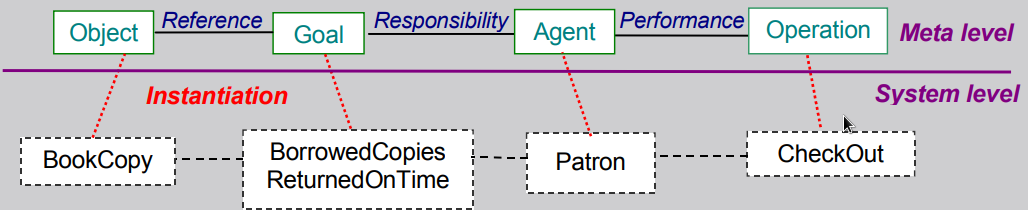
\includegraphics[width=0.9\textwidth]{images/meta-model_rd.png}
    \caption{بازیابی دانش مستقل از دامنه، با استفاده از پارامتر‌های \lr{Objects,
    Goal, Agents, Operation}}
\end{figure}

\subsubsection*{خاص دامنه یا \lr{Domain specific}}

در حقیقت همانطور که از نامش پیداست تماماً و عمیقاً در مورد دامنه صحبت می‌کند تا
بالاترین سطح سازمان.

برای مثال وقتی سیستم مورد نظر نمایشگاه ماشین باشد دامنه‌های آن می‌تواند موارد زیر باشد:

\begin{itemize}
    \item مدیریت نمایشگاه ماشین
    \item مدیریت تحویل و دریافت ماشین‌ها از کمپانی
    \item مدیریت بخش تصادفات
    \item مدیریت بخش بیمه ماشین
\end{itemize}

\subsubsection*{مثال}

سیستم مورد هدف: مدیریت کتابخانه و دامنه: مدیریت منابع

در این مثال منابع در حقیقت کتاب‌ها هستند.

\begin{enumerate}
    \item \lr{Concepts} یا مفاهیم: \begin{enumerate}
        \item منابع (\lr{Resource})
        \item \lr{Resource unit}
        \item \lr{Repository}
        \item \lr{Resource usage}
        \item \lr{Resource availability}
        \item \lr{Resource reservation}
    \end{enumerate}
    \item \lr{Tasks}: \begin{enumerate}
        \item \lr{Tracking the history of resource usage (Like a ledger)}
        \item \lr{Handling resource requests}
    \end{enumerate}
    \item \lr{Actors}: \begin{enumerate}
        \item \lr{Resource users}
        \item \lr{Resource manager}
    \end{enumerate}
    \item \lr{Objectives}: \begin{enumerate}
        \item \lr{Ensuring wide accessibility of resource units to users}
        \item \lr{Ensuring appropriate resource localization in the respoitory
        for easy retrieval}
    \end{enumerate}
    \item \lr{Requirements} یا نیازمندی‌های این سیستم \begin{enumerate}
        \item بررسی حد استفاده منابع به طور مناسب توسط کاربران
        \item تعریف رنج و محدودیت: برای مثال کاربران بیشتر از ۵ کتاب را
        نمی‌توانند از کتابخانه قرض بگیرند.
    \end{enumerate}
    \item \lr{Domain property} یا ویژگی دامنه: \begin{enumerate}
        \item به دلیل آن که کتابخانه فیزیکی است ممکن است از یک کتاب فقط یک نسخه
        موجود باشد، پس وقتی کاربری کتابی را قرض می‌گیرد کاربر دیگر نمی‌تواند
        تقاضای مشابه داشته باشد (یک \lr{fact} می‌باشد).
        \item وقتی کاربری خوش قول نباشد و کتابی به کتابخانه تحویل ندهد، امتیاز
        منفی برای او ثبت می‌شود و از اون جریمه دریافت خواهد شد.
    \end{enumerate}
\end{enumerate}

\subsubsection*{بخش‌هایی که خاص دامنه می‌باشد}

\begin{itemize}
    \item \lr{Resource} $\leftarrow$ \lr{Book}
    \item \lr{Resource unit} $\leftarrow$ \lr{Book copy}
    \item \lr{Repository} $\leftarrow$ \lr{Library shelves}
    \item \lr{User} $\leftarrow$ \lr{Patron}
    \item \lr{Manager} $\leftarrow$ \lr{Library staff}
\end{itemize}

\newpage

\subsection{تکنیک‌های جمع‌آوری اطلاعات ذینفع‌گرا}

بیشتر با انسان‌ها ارتباط دارد تا فرآورده‌هایی که در فرایند مهندسی ممکن است تولید
شوند یا مورد استفاده قرار گیرند.

\subsubsection{\lr{Interviews}}

تمام سوالاتی که برای آن‌ها جوابی نداریم را در بخش \lr{Interview} می‌پرسیم. مثلا
بعد از ثبت‌نام کاربر برای او اعلاناتی ارسال شود؟ یا مثلاً می‌گویم که در سناریو
تغییر کلاس کاربر اعلانات ارسال شود.

در حقیقت برای تمام سوالاتی جوابی نداریم آن‌ها را در بخش \lr{Interview} مطرح
می‌کنیم. پرسش‌نامه به تنهایی کامل نیست، بلکه برای کامل شدنش نیاز به مصاحبه دارد.
معمولاً بدیهیات در مصاحبه پرسیده نمی‌شود.

\begin{enumerate}
    \item ساخت‌یافته: براساس سوال است که پرسیده می‌شود.
    \item بدون ساختار: گفت و گو آزاد و بدون هیچ پیش‌درآمدی می‌باشد.
\end{enumerate}

\subsubsection{\lr{Observation and ethnographic studies}}

در مورد مشاهدات صحبت می‌کند که بیشتر سیستم حال حاضر یا \lr{System-as-is} را مورد
بررسی قرار می‌دهد. هم \lr{Functional requirements} استخراج می‌شوند و هم
\lr{Non-functional requirements}.

این بخش می‌تواند به صورت غیرفعال مانند حالت ناظر باشد یا می‌تواند به صورت فعال
به شکل درگیر شدن با فرآیند‌ها که با یادداشت برداری همراه است باشد.

\subsubsection{\lr{Group sessions}}

\begin{itemize}
    \item ساختار یافته: به هر عضو تیم زمانی داده می‌شود. همه موارد به صورت مشخص
    از پیش تعین شده است. کاملاً نقش هر فردی در تیم مشخص می‌باشد.
    \item بدون ساختار: مانند لحظات طوفان فکری که می‌تواند به شکل نگارش صورت جلسه
    به عنوان نتیجه همفکری‌ها باشد.
    \item بدون سانسور شدن و تمسخر می‌باشد.
\end{itemize}
